\documentclass[1p]{elsarticle_modified}
%\bibliographystyle{elsarticle-num}

%\usepackage[colorlinks]{hyperref}
%\usepackage{abbrmath_seonhwa} %\Abb, \Ascr, \Acal ,\Abf, \Afrak
\usepackage{amsfonts}
\usepackage{amssymb}
\usepackage{amsmath}
\usepackage{amsthm}
\usepackage{scalefnt}
\usepackage{amsbsy}
\usepackage{kotex}
\usepackage{caption}
\usepackage{subfig}
\usepackage{color}
\usepackage{graphicx}
\usepackage{xcolor} %% white, black, red, green, blue, cyan, magenta, yellow
\usepackage{float}
\usepackage{setspace}
\usepackage{hyperref}

\usepackage{tikz}
\usetikzlibrary{arrows}

\usepackage{multirow}
\usepackage{array} % fixed length table
\usepackage{hhline}

%%%%%%%%%%%%%%%%%%%%%
\makeatletter
\renewcommand*\env@matrix[1][\arraystretch]{%
	\edef\arraystretch{#1}%
	\hskip -\arraycolsep
	\let\@ifnextchar\new@ifnextchar
	\array{*\c@MaxMatrixCols c}}
\makeatother %https://tex.stackexchange.com/questions/14071/how-can-i-increase-the-line-spacing-in-a-matrix
%%%%%%%%%%%%%%%

\usepackage[normalem]{ulem}

\newcommand{\msout}[1]{\ifmmode\text{\sout{\ensuremath{#1}}}\else\sout{#1}\fi}
%SOURCE: \msout is \stkout macro in https://tex.stackexchange.com/questions/20609/strikeout-in-math-mode

\newcommand{\cancel}[1]{
	\ifmmode
	{\color{red}\msout{#1}}
	\else
	{\color{red}\sout{#1}}
	\fi
}

\newcommand{\add}[1]{
	{\color{blue}\uwave{#1}}
}

\newcommand{\replace}[2]{
	\ifmmode
	{\color{red}\msout{#1}}{\color{blue}\uwave{#2}}
	\else
	{\color{red}\sout{#1}}{\color{blue}\uwave{#2}}
	\fi
}

\newcommand{\Sol}{\mathcal{S}} %segment
\newcommand{\D}{D} %diagram
\newcommand{\A}{\mathcal{A}} %arc


%%%%%%%%%%%%%%%%%%%%%%%%%%%%%5 test

\def\sl{\operatorname{\textup{SL}}(2,\Cbb)}
\def\psl{\operatorname{\textup{PSL}}(2,\Cbb)}
\def\quan{\mkern 1mu \triangleright \mkern 1mu}

\theoremstyle{definition}
\newtheorem{thm}{Theorem}[section]
\newtheorem{prop}[thm]{Proposition}
\newtheorem{lem}[thm]{Lemma}
\newtheorem{ques}[thm]{Question}
\newtheorem{cor}[thm]{Corollary}
\newtheorem{defn}[thm]{Definition}
\newtheorem{exam}[thm]{Example}
\newtheorem{rmk}[thm]{Remark}
\newtheorem{alg}[thm]{Algorithm}

\newcommand{\I}{\sqrt{-1}}
\begin{document}

%\begin{frontmatter}
%
%\title{Boundary parabolic representations of knots up to 8 crossings}
%
%%% Group authors per affiliation:
%\author{Yunhi Cho} 
%\address{Department of Mathematics, University of Seoul, Seoul, Korea}
%\ead{yhcho@uos.ac.kr}
%
%
%\author{Seonhwa Kim} %\fnref{s_kim}}
%\address{Center for Geometry and Physics, Institute for Basic Science, Pohang, 37673, Korea}
%\ead{ryeona17@ibs.re.kr}
%
%\author{Hyuk Kim}
%\address{Department of Mathematical Sciences, Seoul National University, Seoul 08826, Korea}
%\ead{hyukkim@snu.ac.kr}
%
%\author{Seokbeom Yoon}
%\address{Department of Mathematical Sciences, Seoul National University, Seoul, 08826,  Korea}
%\ead{sbyoon15@snu.ac.kr}
%
%\begin{abstract}
%We find all boundary parabolic representation of knots up to 8 crossings.
%
%\end{abstract}
%\begin{keyword}
%    \MSC[2010] 57M25 
%\end{keyword}
%
%\end{frontmatter}

%\linenumbers
%\tableofcontents
%
\newcommand\colored[1]{\textcolor{white}{\rule[-0.35ex]{0.8em}{1.4ex}}\kern-0.8em\color{red} #1}%
%\newcommand\colored[1]{\textcolor{white}{ #1}\kern-2.17ex	\textcolor{white}{ #1}\kern-1.81ex	\textcolor{white}{ #1}\kern-2.15ex\color{red}#1	}

{\Large $\underline{12a_{0042}~(K12a_{0042})}$}

\setlength{\tabcolsep}{10pt}
\renewcommand{\arraystretch}{1.6}
\vspace{1cm}\begin{tabular}{m{100pt}>{\centering\arraybackslash}m{274pt}}
\multirow{5}{120pt}{
	\centering
	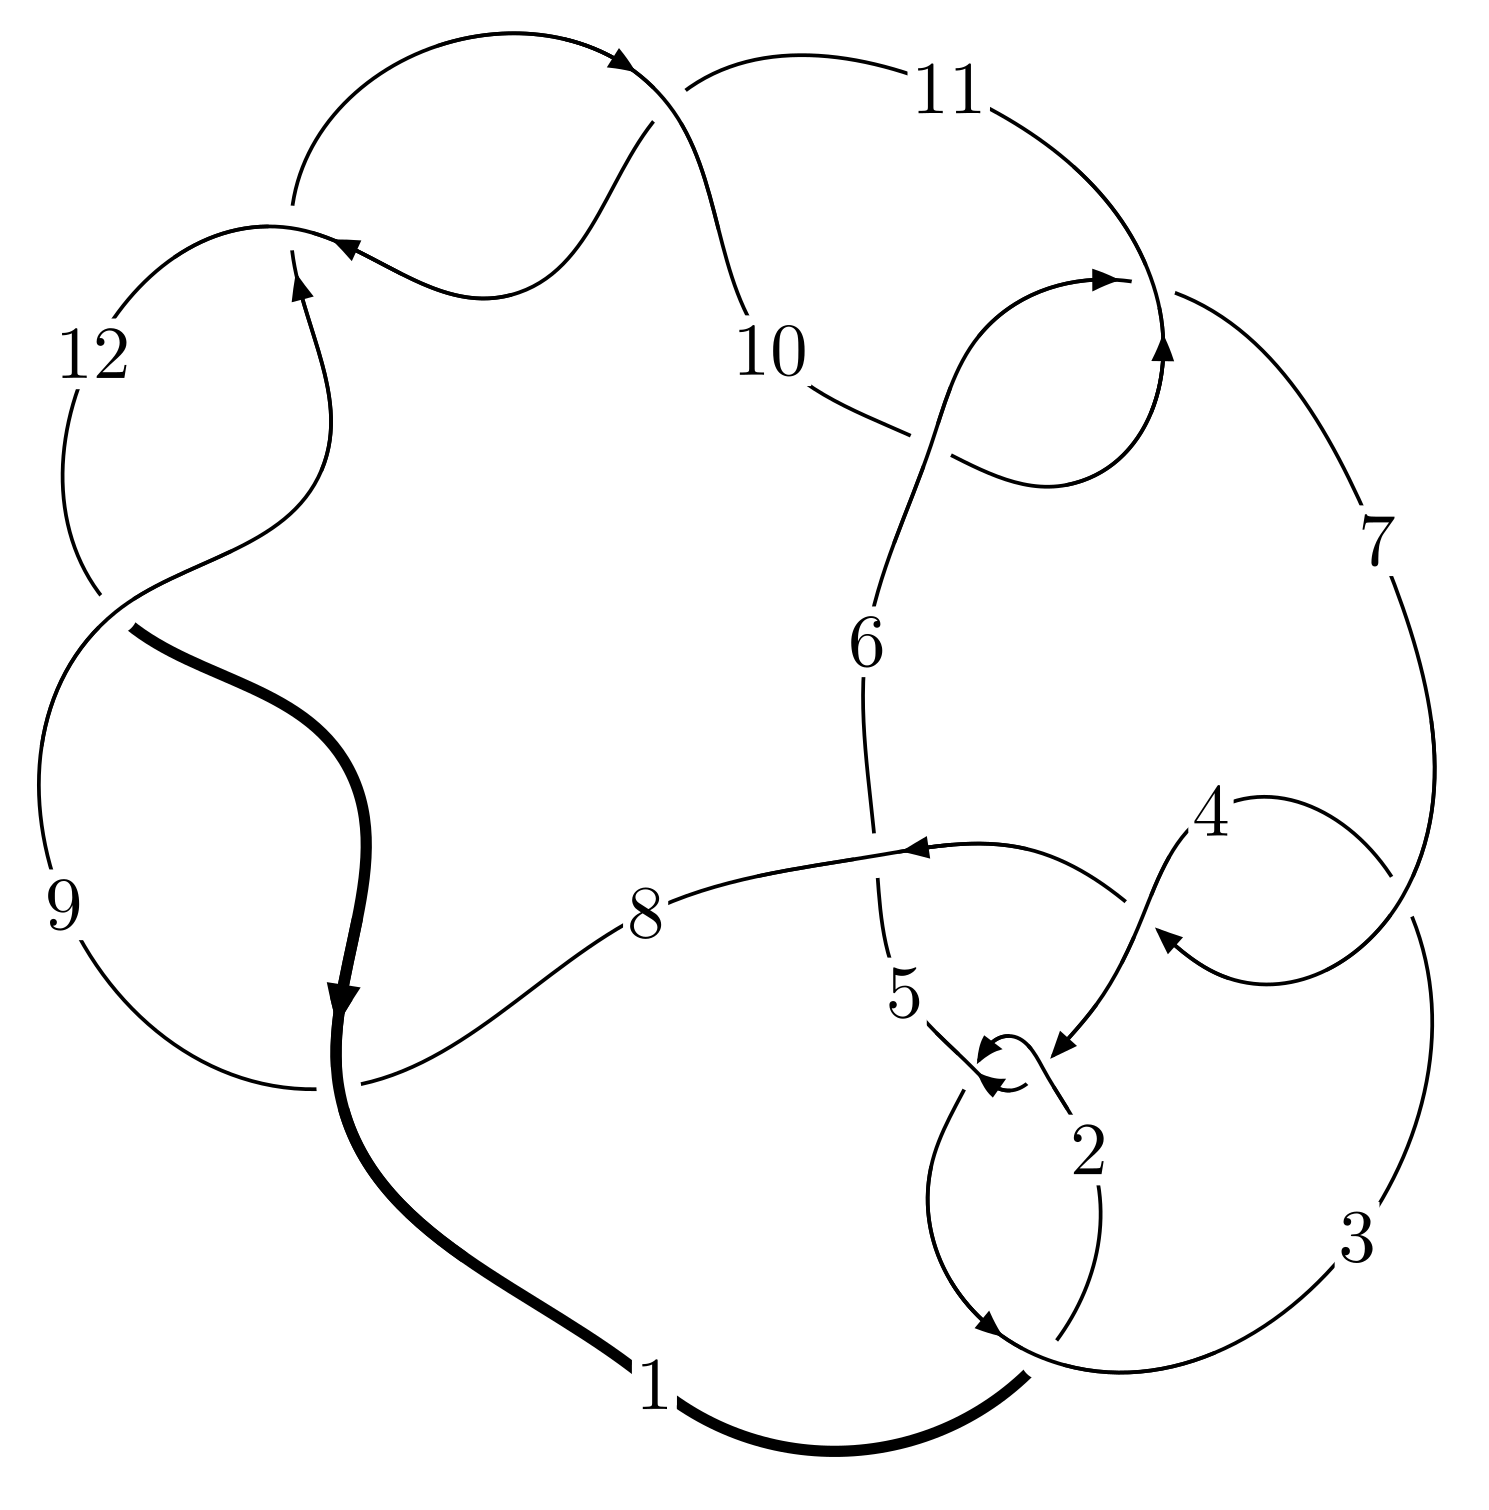
\includegraphics[width=112pt]{../../../GIT/diagram.site/Diagrams/png/843_12a_0042.png}\\
\ \ \ A knot diagram\footnotemark}&
\allowdisplaybreaks
\textbf{Linearized knot diagam} \\
\cline{2-2}
 &
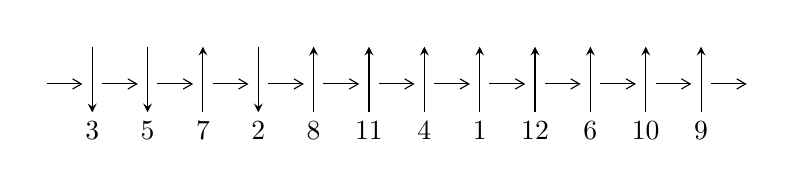
\begin{tikzpicture}[x=20pt, y=17pt]
	% nodes
	\node (C0) at (0, 0) {};
	\node (C1) at (1, 0) {};
	\node (C1U) at (1, +1) {};
	\node (C1D) at (1, -1) {3};

	\node (C2) at (2, 0) {};
	\node (C2U) at (2, +1) {};
	\node (C2D) at (2, -1) {5};

	\node (C3) at (3, 0) {};
	\node (C3U) at (3, +1) {};
	\node (C3D) at (3, -1) {7};

	\node (C4) at (4, 0) {};
	\node (C4U) at (4, +1) {};
	\node (C4D) at (4, -1) {2};

	\node (C5) at (5, 0) {};
	\node (C5U) at (5, +1) {};
	\node (C5D) at (5, -1) {8};

	\node (C6) at (6, 0) {};
	\node (C6U) at (6, +1) {};
	\node (C6D) at (6, -1) {11};

	\node (C7) at (7, 0) {};
	\node (C7U) at (7, +1) {};
	\node (C7D) at (7, -1) {4};

	\node (C8) at (8, 0) {};
	\node (C8U) at (8, +1) {};
	\node (C8D) at (8, -1) {1};

	\node (C9) at (9, 0) {};
	\node (C9U) at (9, +1) {};
	\node (C9D) at (9, -1) {12};

	\node (C10) at (10, 0) {};
	\node (C10U) at (10, +1) {};
	\node (C10D) at (10, -1) {6};

	\node (C11) at (11, 0) {};
	\node (C11U) at (11, +1) {};
	\node (C11D) at (11, -1) {10};

	\node (C12) at (12, 0) {};
	\node (C12U) at (12, +1) {};
	\node (C12D) at (12, -1) {9};
	\node (C13) at (13, 0) {};

	% arrows
	\draw[->,>={angle 60}]
	(C0) edge (C1) (C1) edge (C2) (C2) edge (C3) (C3) edge (C4) (C4) edge (C5) (C5) edge (C6) (C6) edge (C7) (C7) edge (C8) (C8) edge (C9) (C9) edge (C10) (C10) edge (C11) (C11) edge (C12) (C12) edge (C13) ;	\draw[->,>=stealth]
	(C1U) edge (C1D) (C2U) edge (C2D) (C3D) edge (C3U) (C4U) edge (C4D) (C5D) edge (C5U) (C6D) edge (C6U) (C7D) edge (C7U) (C8D) edge (C8U) (C9D) edge (C9U) (C10D) edge (C10U) (C11D) edge (C11U) (C12D) edge (C12U) ;
	\end{tikzpicture} \\
\hhline{~~} \\& 
\textbf{Solving Sequence} \\ \cline{2-2} 
 &
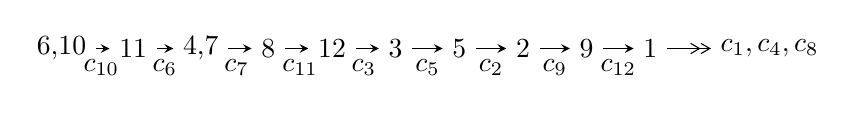
\begin{tikzpicture}[x=23pt, y=7pt]
	% node
	\node (A0) at (-1/8, 0) {6,10};
	\node (A1) at (1, 0) {11};
	\node (A2) at (33/16, 0) {4,7};
	\node (A3) at (25/8, 0) {8};
	\node (A4) at (33/8, 0) {12};
	\node (A5) at (41/8, 0) {3};
	\node (A6) at (49/8, 0) {5};
	\node (A7) at (57/8, 0) {2};
	\node (A8) at (65/8, 0) {9};
	\node (A9) at (73/8, 0) {1};
	\node (C1) at (1/2, -1) {$c_{10}$};
	\node (C2) at (3/2, -1) {$c_{6}$};
	\node (C3) at (21/8, -1) {$c_{7}$};
	\node (C4) at (29/8, -1) {$c_{11}$};
	\node (C5) at (37/8, -1) {$c_{3}$};
	\node (C6) at (45/8, -1) {$c_{5}$};
	\node (C7) at (53/8, -1) {$c_{2}$};
	\node (C8) at (61/8, -1) {$c_{9}$};
	\node (C9) at (69/8, -1) {$c_{12}$};
	\node (A10) at (11, 0) {$c_{1},c_{4},c_{8}$};

	% edge
	\draw[->,>=stealth]	
	(A0) edge (A1) (A1) edge (A2) (A2) edge (A3) (A3) edge (A4) (A4) edge (A5) (A5) edge (A6) (A6) edge (A7) (A7) edge (A8) (A8) edge (A9) ;
	\draw[->>,>={angle 60}]	
	(A9) edge (A10);
\end{tikzpicture} \\ 

\end{tabular} \\

\footnotetext{
The image of knot diagram is generated by the software ``\textbf{Draw programme}" developed by Andrew Bartholomew(\url{http://www.layer8.co.uk/maths/draw/index.htm\#Running-draw}), where we modified some parts for our purpose(\url{https://github.com/CATsTAILs/LinksPainter}).
}\phantom \\ \newline 
\centering \textbf{Ideals for irreducible components\footnotemark of $X_{\text{par}}$} 
 
\begin{align*}
I^u_{1}&=\langle 
u^{69}+u^{68}+\cdots+b-1,\;u^{69}+u^{68}+\cdots+a-1,\;u^{70}+2 u^{69}+\cdots+7 u^3-1\rangle \\
I^u_{2}&=\langle 
- u^4+u^3+b-1,\;- u^4+u^3+a- u-1,\;u^5- u^4+u^2+u-1\rangle \\
\\
\end{align*}
\raggedright * 2 irreducible components of $\dim_{\mathbb{C}}=0$, with total 75 representations.\\
\footnotetext{All coefficients of polynomials are rational numbers. But the coefficients are sometimes approximated in decimal forms when there is not enough margin.}
\newpage
\renewcommand{\arraystretch}{1}
\centering \section*{I. $I^u_{1}= \langle u^{69}+u^{68}+\cdots+b-1,\;u^{69}+u^{68}+\cdots+a-1,\;u^{70}+2 u^{69}+\cdots+7 u^3-1 \rangle$}
\flushleft \textbf{(i) Arc colorings}\\
\begin{tabular}{m{7pt} m{180pt} m{7pt} m{180pt} }
\flushright $a_{6}=$&$\begin{pmatrix}0\\u\end{pmatrix}$ \\
\flushright $a_{10}=$&$\begin{pmatrix}1\\0\end{pmatrix}$ \\
\flushright $a_{11}=$&$\begin{pmatrix}1\\- u^2\end{pmatrix}$ \\
\flushright $a_{4}=$&$\begin{pmatrix}- u^{69}- u^{68}+\cdots+u+1\\- u^{69}- u^{68}+\cdots- u+1\end{pmatrix}$ \\
\flushright $a_{7}=$&$\begin{pmatrix}u\\- u^3+u\end{pmatrix}$ \\
\flushright $a_{8}=$&$\begin{pmatrix}u^8- u^6+3 u^4-2 u^2+1\\u^8+2 u^4\end{pmatrix}$ \\
\flushright $a_{12}=$&$\begin{pmatrix}- u^2+1\\- u^2\end{pmatrix}$ \\
\flushright $a_{3}=$&$\begin{pmatrix}- u^{69}+6 u^{67}+\cdots-2 u^2+2 u\\u^{69}+2 u^{68}+\cdots- u^2-1\end{pmatrix}$ \\
\flushright $a_{5}=$&$\begin{pmatrix}- u^{17}+2 u^{15}-7 u^{13}+10 u^{11}-15 u^9+14 u^7-10 u^5+4 u^3- u\\- u^{17}+u^{15}-5 u^{13}+4 u^{11}-7 u^9+4 u^7-2 u^5+u\end{pmatrix}$ \\
\flushright $a_{2}=$&$\begin{pmatrix}- u^{69}- u^{68}+\cdots+u+1\\- u^{67}+7 u^{65}+\cdots- u^3-2 u^2\end{pmatrix}$ \\
\flushright $a_{9}=$&$\begin{pmatrix}u^4- u^2+1\\u^4\end{pmatrix}$ \\
\flushright $a_{1}=$&$\begin{pmatrix}- u^6+u^4-2 u^2+1\\- u^6- u^2\end{pmatrix}$\\&\end{tabular}
\flushleft \textbf{(ii) Obstruction class $= -1$}\\~\\
\flushleft \textbf{(iii) Cusp Shapes $= 2 u^{69}+3 u^{68}+\cdots+5 u+8$}\\~\\
\newpage\renewcommand{\arraystretch}{1}
\flushleft \textbf{(iv) u-Polynomials at the component}\newline \\
\begin{tabular}{m{50pt}|m{274pt}}
Crossings & \hspace{64pt}u-Polynomials at each crossing \\
\hline $$\begin{aligned}c_{1}\end{aligned}$$&$\begin{aligned}
&u^{70}+34 u^{69}+\cdots+90 u+1
\end{aligned}$\\
\hline $$\begin{aligned}c_{2},c_{4}\end{aligned}$$&$\begin{aligned}
&u^{70}-6 u^{69}+\cdots+10 u-1
\end{aligned}$\\
\hline $$\begin{aligned}c_{3},c_{7}\end{aligned}$$&$\begin{aligned}
&u^{70}- u^{69}+\cdots-160 u+32
\end{aligned}$\\
\hline $$\begin{aligned}c_{5}\end{aligned}$$&$\begin{aligned}
&u^{70}+2 u^{69}+\cdots+1156 u-809
\end{aligned}$\\
\hline $$\begin{aligned}c_{6},c_{10}\end{aligned}$$&$\begin{aligned}
&u^{70}+2 u^{69}+\cdots+7 u^3-1
\end{aligned}$\\
\hline $$\begin{aligned}c_{8},c_{9},c_{11}\\c_{12}\end{aligned}$$&$\begin{aligned}
&u^{70}-14 u^{69}+\cdots-6 u^2+1
\end{aligned}$\\
\hline
\end{tabular}\\~\\
\newpage\renewcommand{\arraystretch}{1}
\flushleft \textbf{(v) Riley Polynomials at the component}\newline \\
\begin{tabular}{m{50pt}|m{274pt}}
Crossings & \hspace{64pt}Riley Polynomials at each crossing \\
\hline $$\begin{aligned}c_{1}\end{aligned}$$&$\begin{aligned}
&y^{70}+10 y^{69}+\cdots-6198 y+1
\end{aligned}$\\
\hline $$\begin{aligned}c_{2},c_{4}\end{aligned}$$&$\begin{aligned}
&y^{70}-34 y^{69}+\cdots-90 y+1
\end{aligned}$\\
\hline $$\begin{aligned}c_{3},c_{7}\end{aligned}$$&$\begin{aligned}
&y^{70}-33 y^{69}+\cdots-19968 y+1024
\end{aligned}$\\
\hline $$\begin{aligned}c_{5}\end{aligned}$$&$\begin{aligned}
&y^{70}+2 y^{69}+\cdots-21431896 y+654481
\end{aligned}$\\
\hline $$\begin{aligned}c_{6},c_{10}\end{aligned}$$&$\begin{aligned}
&y^{70}-14 y^{69}+\cdots-6 y^2+1
\end{aligned}$\\
\hline $$\begin{aligned}c_{8},c_{9},c_{11}\\c_{12}\end{aligned}$$&$\begin{aligned}
&y^{70}+86 y^{69}+\cdots-12 y+1
\end{aligned}$\\
\hline
\end{tabular}\\~\\
\newpage\flushleft \textbf{(vi) Complex Volumes and Cusp Shapes}
$$\begin{array}{c|c|c}  
\text{Solutions to }I^u_{1}& \I (\text{vol} + \sqrt{-1}CS) & \text{Cusp shape}\\
 \hline 
\begin{aligned}
u &= \phantom{-}0.848963 + 0.526476 I \\
a &= -2.22564 + 0.01776 I \\
b &= -2.09137 + 2.15795 I\end{aligned}
 & -2.96182 + 3.57403 I & \phantom{-}4.58642 - 7.96880 I \\ \hline\begin{aligned}
u &= \phantom{-}0.848963 - 0.526476 I \\
a &= -2.22564 - 0.01776 I \\
b &= -2.09137 - 2.15795 I\end{aligned}
 & -2.96182 - 3.57403 I & \phantom{-}4.58642 + 7.96880 I \\ \hline\begin{aligned}
u &= -0.703772 + 0.704213 I \\
a &= \phantom{-}0.381569 - 0.170222 I \\
b &= -0.375365 - 0.155977 I\end{aligned}
 & -3.21240 - 4.24808 I & \phantom{-}2.10319 + 6.98947 I \\ \hline\begin{aligned}
u &= -0.703772 - 0.704213 I \\
a &= \phantom{-}0.381569 + 0.170222 I \\
b &= -0.375365 + 0.155977 I\end{aligned}
 & -3.21240 + 4.24808 I & \phantom{-}2.10319 - 6.98947 I \\ \hline\begin{aligned}
u &= \phantom{-}0.891060 + 0.401648 I \\
a &= \phantom{-}1.315420 - 0.011957 I \\
b &= \phantom{-}1.54143 - 1.57501 I\end{aligned}
 & \phantom{-}3.91808 + 3.09369 I & \phantom{-}11.08096 - 6.18938 I \\ \hline\begin{aligned}
u &= \phantom{-}0.891060 - 0.401648 I \\
a &= \phantom{-}1.315420 + 0.011957 I \\
b &= \phantom{-}1.54143 + 1.57501 I\end{aligned}
 & \phantom{-}3.91808 - 3.09369 I & \phantom{-}11.08096 + 6.18938 I \\ \hline\begin{aligned}
u &= -0.883258 + 0.525678 I \\
a &= -0.476131 + 0.081454 I \\
b &= -0.446033 + 0.623341 I\end{aligned}
 & -2.08503 - 5.95261 I & \phantom{-}3.66675 + 8.33839 I \\ \hline\begin{aligned}
u &= -0.883258 - 0.525678 I \\
a &= -0.476131 - 0.081454 I \\
b &= -0.446033 - 0.623341 I\end{aligned}
 & -2.08503 + 5.95261 I & \phantom{-}3.66675 - 8.33839 I \\ \hline\begin{aligned}
u &= \phantom{-}0.891599 + 0.333493 I \\
a &= -1.009990 + 0.050347 I \\
b &= -1.28724 + 1.45541 I\end{aligned}
 & \phantom{-}2.79991 - 2.14652 I & \phantom{-}9.71265 - 0.23487 I \\ \hline\begin{aligned}
u &= \phantom{-}0.891599 - 0.333493 I \\
a &= -1.009990 - 0.050347 I \\
b &= -1.28724 - 1.45541 I\end{aligned}
 & \phantom{-}2.79991 + 2.14652 I & \phantom{-}9.71265 + 0.23487 I\\
 \hline 
 \end{array}$$\newpage$$\begin{array}{c|c|c}  
\text{Solutions to }I^u_{1}& \I (\text{vol} + \sqrt{-1}CS) & \text{Cusp shape}\\
 \hline 
\begin{aligned}
u &= \phantom{-}0.918259 + 0.512797 I \\
a &= \phantom{-}1.79709 - 0.31181 I \\
b &= \phantom{-}1.65385 - 2.00100 I\end{aligned}
 & \phantom{-}2.56157 + 6.39701 I & \phantom{-}8.79876 - 6.86852 I \\ \hline\begin{aligned}
u &= \phantom{-}0.918259 - 0.512797 I \\
a &= \phantom{-}1.79709 + 0.31181 I \\
b &= \phantom{-}1.65385 + 2.00100 I\end{aligned}
 & \phantom{-}2.56157 - 6.39701 I & \phantom{-}8.79876 + 6.86852 I \\ \hline\begin{aligned}
u &= -0.829178 + 0.656951 I \\
a &= -0.207393 + 0.091221 I \\
b &= \phantom{-}0.224040 + 0.560623 I\end{aligned}
 & -2.80650 - 0.77144 I & \phantom{-0.000000 } 0 \\ \hline\begin{aligned}
u &= -0.829178 - 0.656951 I \\
a &= -0.207393 - 0.091221 I \\
b &= \phantom{-}0.224040 - 0.560623 I\end{aligned}
 & -2.80650 + 0.77144 I & \phantom{-0.000000 } 0 \\ \hline\begin{aligned}
u &= -0.809134 + 0.473685 I \\
a &= \phantom{-}0.493245 + 0.198012 I \\
b &= \phantom{-}0.542821 - 0.286131 I\end{aligned}
 & -0.89626 - 1.96724 I & \phantom{-}5.61742 + 3.44733 I \\ \hline\begin{aligned}
u &= -0.809134 - 0.473685 I \\
a &= \phantom{-}0.493245 - 0.198012 I \\
b &= \phantom{-}0.542821 + 0.286131 I\end{aligned}
 & -0.89626 + 1.96724 I & \phantom{-}5.61742 - 3.44733 I \\ \hline\begin{aligned}
u &= -0.925343 + 0.107219 I \\
a &= \phantom{-}1.68417 + 0.13957 I \\
b &= \phantom{-}1.58116 - 0.07754 I\end{aligned}
 & \phantom{-}4.00519 - 7.11466 I & \phantom{-}11.47294 + 7.09856 I \\ \hline\begin{aligned}
u &= -0.925343 - 0.107219 I \\
a &= \phantom{-}1.68417 - 0.13957 I \\
b &= \phantom{-}1.58116 + 0.07754 I\end{aligned}
 & \phantom{-}4.00519 + 7.11466 I & \phantom{-}11.47294 - 7.09856 I \\ \hline\begin{aligned}
u &= \phantom{-}0.933419 + 0.540532 I \\
a &= -1.82278 + 0.45018 I \\
b &= -1.56950 + 2.06664 I\end{aligned}
 & \phantom{-}0.36752 + 11.87470 I & \phantom{-0.000000 } 0. - 10.68011 I \\ \hline\begin{aligned}
u &= \phantom{-}0.933419 - 0.540532 I \\
a &= -1.82278 - 0.45018 I \\
b &= -1.56950 - 2.06664 I\end{aligned}
 & \phantom{-}0.36752 - 11.87470 I & \phantom{-0.000000 -}0. + 10.68011 I\\
 \hline 
 \end{array}$$\newpage$$\begin{array}{c|c|c}  
\text{Solutions to }I^u_{1}& \I (\text{vol} + \sqrt{-1}CS) & \text{Cusp shape}\\
 \hline 
\begin{aligned}
u &= -0.913045 + 0.060749 I \\
a &= -1.77668 - 0.10528 I \\
b &= -1.62183 + 0.02869 I\end{aligned}
 & \phantom{-}5.72534 - 1.70594 I & \phantom{-}14.7293 + 1.6894 I \\ \hline\begin{aligned}
u &= -0.913045 - 0.060749 I \\
a &= -1.77668 + 0.10528 I \\
b &= -1.62183 - 0.02869 I\end{aligned}
 & \phantom{-}5.72534 + 1.70594 I & \phantom{-}14.7293 - 1.6894 I \\ \hline\begin{aligned}
u &= \phantom{-}0.510558 + 0.701915 I \\
a &= -0.49728 + 1.97299 I \\
b &= \phantom{-}0.99266 + 1.29279 I\end{aligned}
 & -1.00091 - 7.27047 I & \phantom{-}1.97102 + 4.94885 I \\ \hline\begin{aligned}
u &= \phantom{-}0.510558 - 0.701915 I \\
a &= -0.49728 - 1.97299 I \\
b &= \phantom{-}0.99266 - 1.29279 I\end{aligned}
 & -1.00091 + 7.27047 I & \phantom{-}1.97102 - 4.94885 I \\ \hline\begin{aligned}
u &= -0.682836 + 0.516888 I \\
a &= \phantom{-}0.113681 + 0.487864 I \\
b &= \phantom{-}0.399773 + 0.054104 I\end{aligned}
 & -1.31076 - 1.82986 I & \phantom{-}3.73022 + 5.65801 I \\ \hline\begin{aligned}
u &= -0.682836 - 0.516888 I \\
a &= \phantom{-}0.113681 - 0.487864 I \\
b &= \phantom{-}0.399773 - 0.054104 I\end{aligned}
 & -1.31076 + 1.82986 I & \phantom{-}3.73022 - 5.65801 I \\ \hline\begin{aligned}
u &= \phantom{-}0.605074 + 0.592671 I \\
a &= -0.09109 + 2.15794 I \\
b &= \phantom{-}1.70767 + 1.21369 I\end{aligned}
 & -3.74961 + 0.67285 I & \phantom{-}0.349013 + 0.900580 I \\ \hline\begin{aligned}
u &= \phantom{-}0.605074 - 0.592671 I \\
a &= -0.09109 - 2.15794 I \\
b &= \phantom{-}1.70767 - 1.21369 I\end{aligned}
 & -3.74961 - 0.67285 I & \phantom{-}0.349013 - 0.900580 I \\ \hline\begin{aligned}
u &= \phantom{-}0.844028 + 0.060120 I \\
a &= -0.134807 + 0.151297 I \\
b &= -0.241531 + 1.133100 I\end{aligned}
 & \phantom{-}1.03953 + 1.86544 I & \phantom{-}10.82292 - 4.22163 I \\ \hline\begin{aligned}
u &= \phantom{-}0.844028 - 0.060120 I \\
a &= -0.134807 - 0.151297 I \\
b &= -0.241531 - 1.133100 I\end{aligned}
 & \phantom{-}1.03953 - 1.86544 I & \phantom{-}10.82292 + 4.22163 I\\
 \hline 
 \end{array}$$\newpage$$\begin{array}{c|c|c}  
\text{Solutions to }I^u_{1}& \I (\text{vol} + \sqrt{-1}CS) & \text{Cusp shape}\\
 \hline 
\begin{aligned}
u &= -0.550080 + 0.618252 I \\
a &= \phantom{-}0.389492 - 0.684495 I \\
b &= -0.292647 - 0.181492 I\end{aligned}
 & -3.14503 + 1.63469 I & -0.27409 - 1.40763 I \\ \hline\begin{aligned}
u &= -0.550080 - 0.618252 I \\
a &= \phantom{-}0.389492 + 0.684495 I \\
b &= -0.292647 + 0.181492 I\end{aligned}
 & -3.14503 - 1.63469 I & -0.27409 + 1.40763 I \\ \hline\begin{aligned}
u &= \phantom{-}0.482045 + 0.648946 I \\
a &= \phantom{-}0.44168 - 1.88279 I \\
b &= -1.04226 - 1.10595 I\end{aligned}
 & \phantom{-}1.18543 - 2.05480 I & \phantom{-}5.19934 + 0.85632 I \\ \hline\begin{aligned}
u &= \phantom{-}0.482045 - 0.648946 I \\
a &= \phantom{-}0.44168 + 1.88279 I \\
b &= -1.04226 + 1.10595 I\end{aligned}
 & \phantom{-}1.18543 + 2.05480 I & \phantom{-}5.19934 - 0.85632 I \\ \hline\begin{aligned}
u &= -0.786558\phantom{ +0.000000I} \\
a &= \phantom{-}2.34128\phantom{ +0.000000I} \\
b &= \phantom{-}1.76553\phantom{ +0.000000I}\end{aligned}
 & -0.192753\phantom{ +0.000000I} & \phantom{-}15.7720\phantom{ +0.000000I} \\ \hline\begin{aligned}
u &= -0.896752 + 0.854059 I \\
a &= \phantom{-}0.459172 - 0.811143 I \\
b &= \phantom{-}2.34273 + 0.72734 I\end{aligned}
 & -3.69892 - 0.39441 I & \phantom{-0.000000 } 0 \\ \hline\begin{aligned}
u &= -0.896752 - 0.854059 I \\
a &= \phantom{-}0.459172 + 0.811143 I \\
b &= \phantom{-}2.34273 - 0.72734 I\end{aligned}
 & -3.69892 + 0.39441 I & \phantom{-0.000000 } 0 \\ \hline\begin{aligned}
u &= -0.929010 + 0.846151 I \\
a &= -0.927478 + 0.420395 I \\
b &= -2.24639 - 1.74550 I\end{aligned}
 & -3.60036 - 5.92816 I & \phantom{-0.000000 } 0 \\ \hline\begin{aligned}
u &= -0.929010 - 0.846151 I \\
a &= -0.927478 - 0.420395 I \\
b &= -2.24639 + 1.74550 I\end{aligned}
 & -3.60036 + 5.92816 I & \phantom{-0.000000 } 0 \\ \hline\begin{aligned}
u &= -0.888018 + 0.909430 I \\
a &= -0.29657 - 1.69935 I \\
b &= \phantom{-}2.75886 - 1.26977 I\end{aligned}
 & -6.66789 + 2.80518 I & \phantom{-0.000000 } 0\\
 \hline 
 \end{array}$$\newpage$$\begin{array}{c|c|c}  
\text{Solutions to }I^u_{1}& \I (\text{vol} + \sqrt{-1}CS) & \text{Cusp shape}\\
 \hline 
\begin{aligned}
u &= -0.888018 - 0.909430 I \\
a &= -0.29657 + 1.69935 I \\
b &= \phantom{-}2.75886 + 1.26977 I\end{aligned}
 & -6.66789 - 2.80518 I & \phantom{-0.000000 } 0 \\ \hline\begin{aligned}
u &= \phantom{-}0.911261 + 0.892581 I \\
a &= -0.290253 + 0.624136 I \\
b &= \phantom{-}0.068856 + 0.705184 I\end{aligned}
 & -9.41866 + 2.57034 I & \phantom{-0.000000 } 0 \\ \hline\begin{aligned}
u &= \phantom{-}0.911261 - 0.892581 I \\
a &= -0.290253 - 0.624136 I \\
b &= \phantom{-}0.068856 - 0.705184 I\end{aligned}
 & -9.41866 - 2.57034 I & \phantom{-0.000000 } 0 \\ \hline\begin{aligned}
u &= \phantom{-}0.898692 + 0.907339 I \\
a &= \phantom{-}0.140709 - 0.798542 I \\
b &= -0.287738 - 0.771476 I\end{aligned}
 & -11.28450 - 1.94871 I & \phantom{-0.000000 } 0 \\ \hline\begin{aligned}
u &= \phantom{-}0.898692 - 0.907339 I \\
a &= \phantom{-}0.140709 + 0.798542 I \\
b &= -0.287738 + 0.771476 I\end{aligned}
 & -11.28450 + 1.94871 I & \phantom{-0.000000 } 0 \\ \hline\begin{aligned}
u &= -0.905732 + 0.903520 I \\
a &= -0.07637 + 2.14749 I \\
b &= -3.85473 + 1.23788 I\end{aligned}
 & -12.02480 - 0.74463 I & \phantom{-0.000000 } 0 \\ \hline\begin{aligned}
u &= -0.905732 - 0.903520 I \\
a &= -0.07637 - 2.14749 I \\
b &= -3.85473 - 1.23788 I\end{aligned}
 & -12.02480 + 0.74463 I & \phantom{-0.000000 } 0 \\ \hline\begin{aligned}
u &= -0.889133 + 0.920620 I \\
a &= \phantom{-}0.53328 + 1.76854 I \\
b &= -2.56436 + 1.69325 I\end{aligned}
 & -9.24667 + 8.31125 I & \phantom{-0.000000 } 0 \\ \hline\begin{aligned}
u &= -0.889133 - 0.920620 I \\
a &= \phantom{-}0.53328 - 1.76854 I \\
b &= -2.56436 - 1.69325 I\end{aligned}
 & -9.24667 - 8.31125 I & \phantom{-0.000000 } 0 \\ \hline\begin{aligned}
u &= \phantom{-}0.940923 + 0.878414 I \\
a &= -0.602531 + 0.307679 I \\
b &= -0.386679 + 0.597282 I\end{aligned}
 & -9.32294 + 3.97310 I & \phantom{-0.000000 } 0\\
 \hline 
 \end{array}$$\newpage$$\begin{array}{c|c|c}  
\text{Solutions to }I^u_{1}& \I (\text{vol} + \sqrt{-1}CS) & \text{Cusp shape}\\
 \hline 
\begin{aligned}
u &= \phantom{-}0.940923 - 0.878414 I \\
a &= -0.602531 - 0.307679 I \\
b &= -0.386679 - 0.597282 I\end{aligned}
 & -9.32294 - 3.97310 I & \phantom{-0.000000 } 0 \\ \hline\begin{aligned}
u &= -0.951721 + 0.881216 I \\
a &= \phantom{-}2.16536 - 0.07906 I \\
b &= \phantom{-}2.78923 + 3.81036 I\end{aligned}
 & -11.87630 - 5.84179 I & \phantom{-0.000000 } 0 \\ \hline\begin{aligned}
u &= -0.951721 - 0.881216 I \\
a &= \phantom{-}2.16536 + 0.07906 I \\
b &= \phantom{-}2.78923 - 3.81036 I\end{aligned}
 & -11.87630 + 5.84179 I & \phantom{-0.000000 } 0 \\ \hline\begin{aligned}
u &= \phantom{-}0.958325 + 0.878505 I \\
a &= \phantom{-}0.755872 - 0.166096 I \\
b &= \phantom{-}0.610563 - 0.547751 I\end{aligned}
 & -11.09220 + 8.53782 I & \phantom{-0.000000 } 0 \\ \hline\begin{aligned}
u &= \phantom{-}0.958325 - 0.878505 I \\
a &= \phantom{-}0.755872 + 0.166096 I \\
b &= \phantom{-}0.610563 + 0.547751 I\end{aligned}
 & -11.09220 - 8.53782 I & \phantom{-0.000000 } 0 \\ \hline\begin{aligned}
u &= -0.965439 + 0.872470 I \\
a &= -1.71394 - 0.28873 I \\
b &= -1.90629 - 3.41650 I\end{aligned}
 & -6.41881 - 9.38008 I & \phantom{-0.000000 } 0 \\ \hline\begin{aligned}
u &= -0.965439 - 0.872470 I \\
a &= -1.71394 + 0.28873 I \\
b &= -1.90629 + 3.41650 I\end{aligned}
 & -6.41881 + 9.38008 I & \phantom{-0.000000 } 0 \\ \hline\begin{aligned}
u &= \phantom{-}0.928310 + 0.917655 I \\
a &= -0.170687 - 0.499826 I \\
b &= -0.403670 - 0.360916 I\end{aligned}
 & -12.77690 + 4.46172 I & \phantom{-0.000000 } 0 \\ \hline\begin{aligned}
u &= \phantom{-}0.928310 - 0.917655 I \\
a &= -0.170687 + 0.499826 I \\
b &= -0.403670 + 0.360916 I\end{aligned}
 & -12.77690 - 4.46172 I & \phantom{-0.000000 } 0 \\ \hline\begin{aligned}
u &= -0.972378 + 0.878766 I \\
a &= \phantom{-}1.76827 + 0.52427 I \\
b &= \phantom{-}1.60446 + 3.65424 I\end{aligned}
 & -8.9768 - 14.9420 I & \phantom{-0.000000 } 0\\
 \hline 
 \end{array}$$\newpage$$\begin{array}{c|c|c}  
\text{Solutions to }I^u_{1}& \I (\text{vol} + \sqrt{-1}CS) & \text{Cusp shape}\\
 \hline 
\begin{aligned}
u &= -0.972378 - 0.878766 I \\
a &= \phantom{-}1.76827 - 0.52427 I \\
b &= \phantom{-}1.60446 - 3.65424 I\end{aligned}
 & -8.9768 + 14.9420 I & \phantom{-0.000000 } 0 \\ \hline\begin{aligned}
u &= \phantom{-}0.949802 + 0.906372 I \\
a &= \phantom{-}0.487273 + 0.146616 I \\
b &= \phantom{-}0.517570 - 0.112853 I\end{aligned}
 & -12.70680 + 2.25291 I & \phantom{-0.000000 } 0 \\ \hline\begin{aligned}
u &= \phantom{-}0.949802 - 0.906372 I \\
a &= \phantom{-}0.487273 - 0.146616 I \\
b &= \phantom{-}0.517570 + 0.112853 I\end{aligned}
 & -12.70680 - 2.25291 I & \phantom{-0.000000 } 0 \\ \hline\begin{aligned}
u &= \phantom{-}0.259476 + 0.549278 I \\
a &= \phantom{-}0.69911 - 1.56843 I \\
b &= -0.640976 - 0.684812 I\end{aligned}
 & \phantom{-}2.10455 + 0.34368 I & \phantom{-}5.70795 - 0.43243 I \\ \hline\begin{aligned}
u &= \phantom{-}0.259476 - 0.549278 I \\
a &= \phantom{-}0.69911 + 1.56843 I \\
b &= -0.640976 + 0.684812 I\end{aligned}
 & \phantom{-}2.10455 - 0.34368 I & \phantom{-}5.70795 + 0.43243 I \\ \hline\begin{aligned}
u &= \phantom{-}0.150083 + 0.588539 I \\
a &= -0.81656 + 1.59215 I \\
b &= \phantom{-}0.461872 + 0.688311 I\end{aligned}
 & \phantom{-}0.54630 + 5.24919 I & \phantom{-}2.36877 - 5.53828 I \\ \hline\begin{aligned}
u &= \phantom{-}0.150083 - 0.588539 I \\
a &= -0.81656 - 1.59215 I \\
b &= \phantom{-}0.461872 - 0.688311 I\end{aligned}
 & \phantom{-}0.54630 - 5.24919 I & \phantom{-}2.36877 + 5.53828 I \\ \hline\begin{aligned}
u &= \phantom{-}0.577939\phantom{ +0.000000I} \\
a &= \phantom{-}0.191919\phantom{ +0.000000I} \\
b &= -0.448397\phantom{ +0.000000I}\end{aligned}
 & \phantom{-}0.745390\phantom{ +0.000000I} & \phantom{-}14.0380\phantom{ +0.000000I} \\ \hline\begin{aligned}
u &= -0.122739 + 0.348425 I \\
a &= -0.75582 + 1.74701 I \\
b &= \phantom{-}0.302481 + 0.442001 I\end{aligned}
 & -1.73126 - 0.78637 I & -2.82494 + 1.32713 I \\ \hline\begin{aligned}
u &= -0.122739 - 0.348425 I \\
a &= -0.75582 - 1.74701 I \\
b &= \phantom{-}0.302481 - 0.442001 I\end{aligned}
 & -1.73126 + 0.78637 I & -2.82494 - 1.32713 I\\
 \hline 
 \end{array}$$\newpage\newpage\renewcommand{\arraystretch}{1}
\centering \section*{II. $I^u_{2}= \langle - u^4+u^3+b-1,\;- u^4+u^3+a- u-1,\;u^5- u^4+u^2+u-1 \rangle$}
\flushleft \textbf{(i) Arc colorings}\\
\begin{tabular}{m{7pt} m{180pt} m{7pt} m{180pt} }
\flushright $a_{6}=$&$\begin{pmatrix}0\\u\end{pmatrix}$ \\
\flushright $a_{10}=$&$\begin{pmatrix}1\\0\end{pmatrix}$ \\
\flushright $a_{11}=$&$\begin{pmatrix}1\\- u^2\end{pmatrix}$ \\
\flushright $a_{4}=$&$\begin{pmatrix}u^4- u^3+u+1\\u^4- u^3+1\end{pmatrix}$ \\
\flushright $a_{7}=$&$\begin{pmatrix}u\\- u^3+u\end{pmatrix}$ \\
\flushright $a_{8}=$&$\begin{pmatrix}u\\- u^3+u\end{pmatrix}$ \\
\flushright $a_{12}=$&$\begin{pmatrix}- u^2+1\\- u^2\end{pmatrix}$ \\
\flushright $a_{3}=$&$\begin{pmatrix}u^4- u^3+u+1\\u^4- u^3+1\end{pmatrix}$ \\
\flushright $a_{5}=$&$\begin{pmatrix}- u^3\\u^4- u^3- u^2+1\end{pmatrix}$ \\
\flushright $a_{2}=$&$\begin{pmatrix}u^4+u+1\\u^2\end{pmatrix}$ \\
\flushright $a_{9}=$&$\begin{pmatrix}u^4- u^2+1\\u^4\end{pmatrix}$ \\
\flushright $a_{1}=$&$\begin{pmatrix}u^3\\- u^4+u^3+u^2-1\end{pmatrix}$\\&\end{tabular}
\flushleft \textbf{(ii) Obstruction class $= 1$}\\~\\
\flushleft \textbf{(iii) Cusp Shapes $= u^3-3 u^2+u+2$}\\~\\
\newpage\renewcommand{\arraystretch}{1}
\flushleft \textbf{(iv) u-Polynomials at the component}\newline \\
\begin{tabular}{m{50pt}|m{274pt}}
Crossings & \hspace{64pt}u-Polynomials at each crossing \\
\hline $$\begin{aligned}c_{1},c_{2}\end{aligned}$$&$\begin{aligned}
&(u-1)^5
\end{aligned}$\\
\hline $$\begin{aligned}c_{3},c_{7}\end{aligned}$$&$\begin{aligned}
&u^5
\end{aligned}$\\
\hline $$\begin{aligned}c_{4}\end{aligned}$$&$\begin{aligned}
&(u+1)^5
\end{aligned}$\\
\hline $$\begin{aligned}c_{5},c_{8},c_{9}\end{aligned}$$&$\begin{aligned}
&u^5+u^4+4 u^3+3 u^2+3 u+1
\end{aligned}$\\
\hline $$\begin{aligned}c_{6}\end{aligned}$$&$\begin{aligned}
&u^5+u^4- u^2+u+1
\end{aligned}$\\
\hline $$\begin{aligned}c_{10}\end{aligned}$$&$\begin{aligned}
&u^5- u^4+u^2+u-1
\end{aligned}$\\
\hline $$\begin{aligned}c_{11},c_{12}\end{aligned}$$&$\begin{aligned}
&u^5- u^4+4 u^3-3 u^2+3 u-1
\end{aligned}$\\
\hline
\end{tabular}\\~\\
\newpage\renewcommand{\arraystretch}{1}
\flushleft \textbf{(v) Riley Polynomials at the component}\newline \\
\begin{tabular}{m{50pt}|m{274pt}}
Crossings & \hspace{64pt}Riley Polynomials at each crossing \\
\hline $$\begin{aligned}c_{1},c_{2},c_{4}\end{aligned}$$&$\begin{aligned}
&(y-1)^5
\end{aligned}$\\
\hline $$\begin{aligned}c_{3},c_{7}\end{aligned}$$&$\begin{aligned}
&y^5
\end{aligned}$\\
\hline $$\begin{aligned}c_{5},c_{8},c_{9}\\c_{11},c_{12}\end{aligned}$$&$\begin{aligned}
&y^5+7 y^4+16 y^3+13 y^2+3 y-1
\end{aligned}$\\
\hline $$\begin{aligned}c_{6},c_{10}\end{aligned}$$&$\begin{aligned}
&y^5- y^4+4 y^3-3 y^2+3 y-1
\end{aligned}$\\
\hline
\end{tabular}\\~\\
\newpage\flushleft \textbf{(vi) Complex Volumes and Cusp Shapes}
$$\begin{array}{c|c|c}  
\text{Solutions to }I^u_{2}& \I (\text{vol} + \sqrt{-1}CS) & \text{Cusp shape}\\
 \hline 
\begin{aligned}
u &= -0.758138 + 0.584034 I \\
a &= -0.827780 - 0.637683 I \\
b &= -0.069642 - 1.221720 I\end{aligned}
 & -3.46474 - 2.21397 I & \phantom{-}0.88087 + 4.04855 I \\ \hline\begin{aligned}
u &= -0.758138 - 0.584034 I \\
a &= -0.827780 + 0.637683 I \\
b &= -0.069642 + 1.221720 I\end{aligned}
 & -3.46474 + 2.21397 I & \phantom{-}0.88087 - 4.04855 I \\ \hline\begin{aligned}
u &= \phantom{-}0.935538 + 0.903908 I \\
a &= \phantom{-}0.552827 - 0.534136 I \\
b &= -0.38271 - 1.43804 I\end{aligned}
 & -12.60320 + 3.33174 I & \phantom{-}1.28666 - 2.53508 I \\ \hline\begin{aligned}
u &= \phantom{-}0.935538 - 0.903908 I \\
a &= \phantom{-}0.552827 + 0.534136 I \\
b &= -0.38271 + 1.43804 I\end{aligned}
 & -12.60320 - 3.33174 I & \phantom{-}1.28666 + 2.53508 I \\ \hline\begin{aligned}
u &= \phantom{-}0.645200\phantom{ +0.000000I} \\
a &= \phantom{-}1.54991\phantom{ +0.000000I} \\
b &= \phantom{-}0.904706\phantom{ +0.000000I}\end{aligned}
 & -0.762751\phantom{ +0.000000I} & \phantom{-}1.66490\phantom{ +0.000000I}\\
 \hline 
 \end{array}$$\newpage
\newpage\renewcommand{\arraystretch}{1}
\centering \section*{ III. u-Polynomials}
\begin{tabular}{m{50pt}|m{274pt}}
Crossings & \hspace{64pt}u-Polynomials at each crossing \\
\hline $$\begin{aligned}c_{1}\end{aligned}$$&$\begin{aligned}
&((u-1)^5)(u^{70}+34 u^{69}+\cdots+90 u+1)
\end{aligned}$\\
\hline $$\begin{aligned}c_{2}\end{aligned}$$&$\begin{aligned}
&((u-1)^5)(u^{70}-6 u^{69}+\cdots+10 u-1)
\end{aligned}$\\
\hline $$\begin{aligned}c_{3},c_{7}\end{aligned}$$&$\begin{aligned}
&u^5(u^{70}- u^{69}+\cdots-160 u+32)
\end{aligned}$\\
\hline $$\begin{aligned}c_{4}\end{aligned}$$&$\begin{aligned}
&((u+1)^5)(u^{70}-6 u^{69}+\cdots+10 u-1)
\end{aligned}$\\
\hline $$\begin{aligned}c_{5}\end{aligned}$$&$\begin{aligned}
&(u^5+u^4+4 u^3+3 u^2+3 u+1)(u^{70}+2 u^{69}+\cdots+1156 u-809)
\end{aligned}$\\
\hline $$\begin{aligned}c_{6}\end{aligned}$$&$\begin{aligned}
&(u^5+u^4- u^2+u+1)(u^{70}+2 u^{69}+\cdots+7 u^3-1)
\end{aligned}$\\
\hline $$\begin{aligned}c_{8},c_{9}\end{aligned}$$&$\begin{aligned}
&(u^5+u^4+4 u^3+3 u^2+3 u+1)(u^{70}-14 u^{69}+\cdots-6 u^2+1)
\end{aligned}$\\
\hline $$\begin{aligned}c_{10}\end{aligned}$$&$\begin{aligned}
&(u^5- u^4+u^2+u-1)(u^{70}+2 u^{69}+\cdots+7 u^3-1)
\end{aligned}$\\
\hline $$\begin{aligned}c_{11},c_{12}\end{aligned}$$&$\begin{aligned}
&(u^5- u^4+4 u^3-3 u^2+3 u-1)(u^{70}-14 u^{69}+\cdots-6 u^2+1)
\end{aligned}$\\
\hline
\end{tabular}\newpage\renewcommand{\arraystretch}{1}
\centering \section*{ IV. Riley Polynomials}
\begin{tabular}{m{50pt}|m{274pt}}
Crossings & \hspace{64pt}Riley Polynomials at each crossing \\
\hline $$\begin{aligned}c_{1}\end{aligned}$$&$\begin{aligned}
&((y-1)^5)(y^{70}+10 y^{69}+\cdots-6198 y+1)
\end{aligned}$\\
\hline $$\begin{aligned}c_{2},c_{4}\end{aligned}$$&$\begin{aligned}
&((y-1)^5)(y^{70}-34 y^{69}+\cdots-90 y+1)
\end{aligned}$\\
\hline $$\begin{aligned}c_{3},c_{7}\end{aligned}$$&$\begin{aligned}
&y^5(y^{70}-33 y^{69}+\cdots-19968 y+1024)
\end{aligned}$\\
\hline $$\begin{aligned}c_{5}\end{aligned}$$&$\begin{aligned}
&(y^5+7 y^4+16 y^3+13 y^2+3 y-1)\\
&\cdot(y^{70}+2 y^{69}+\cdots-21431896 y+654481)
\end{aligned}$\\
\hline $$\begin{aligned}c_{6},c_{10}\end{aligned}$$&$\begin{aligned}
&(y^5- y^4+4 y^3-3 y^2+3 y-1)(y^{70}-14 y^{69}+\cdots-6 y^2+1)
\end{aligned}$\\
\hline $$\begin{aligned}c_{8},c_{9},c_{11}\\c_{12}\end{aligned}$$&$\begin{aligned}
&(y^5+7 y^4+16 y^3+13 y^2+3 y-1)(y^{70}+86 y^{69}+\cdots-12 y+1)
\end{aligned}$\\
\hline
\end{tabular}
\vskip 2pc
\end{document}